%!TEX root = ../template.tex
%%%%%%%%%%%%%%%%%%%%%%%%%%%%%%%%%%%%%%%%%%%%%%%%%%%%%%%%%%%%%%%%%%%%
%% chapter4.tex
%% NOVA thesis document file
%%
%% Chapter with a short latex tutorial and examples
%%%%%%%%%%%%%%%%%%%%%%%%%%%%%%%%%%%%%%%%%%%%%%%%%%%%%%%%%%%%%%%%%%%%

\typeout{NT FILE chapter4.tex}%

\chapter{Population recordings of cerebellar neurons show a variety of modulations by locomotion}
\label{cha:locopixels}

\section{Abstract}
\section{Introduction}
\begin{itemize}
    \item motivate simultaneous population recordings
    \item a hypothesis about cerebellar funnction during locomotion?
\end{itemize}

\section{Results}
\subsection{Cerebellar neurons show a variety of responses to locomotor events}

\begin{figure}[h]
    \centering
    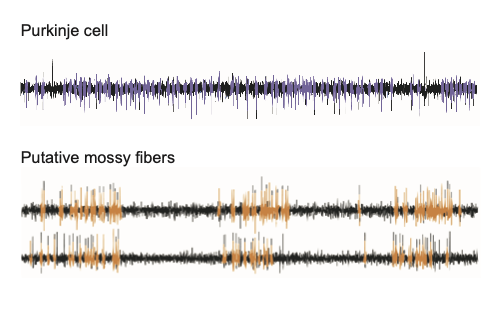
\includegraphics[width=.7\linewidth]{Chapters//Figures//chapter5/pkj_mossy_raw.png}
    \caption{Enter Caption}
    \label{fig:raw_channels}
\end{figure}

\subsection{Mossy fibers and Purkinje cells have distinct firing modulations by behavior}

\begin{figure}[h]
    \centering
    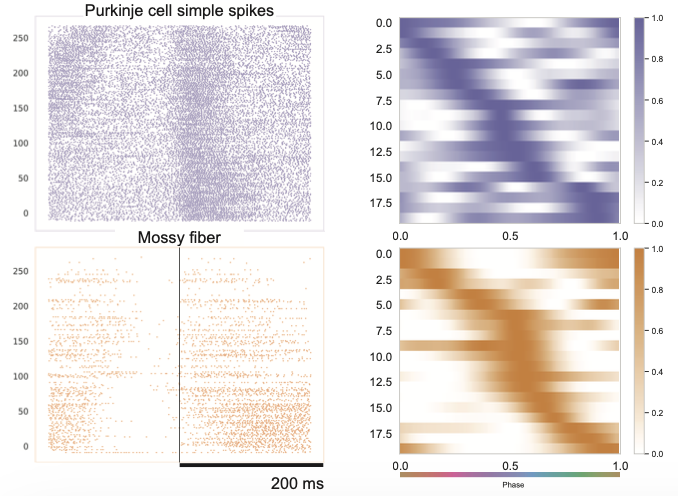
\includegraphics[width=.7\linewidth]{Chapters//Figures//chapter5/pkj_mossy_tuning.png}
    \caption{Enter Caption}
    \label{fig:pop_tuning}
\end{figure}

\subsection{Behavior can be decoded from both populations at different delays?}


\begin{figure}
    \centering
    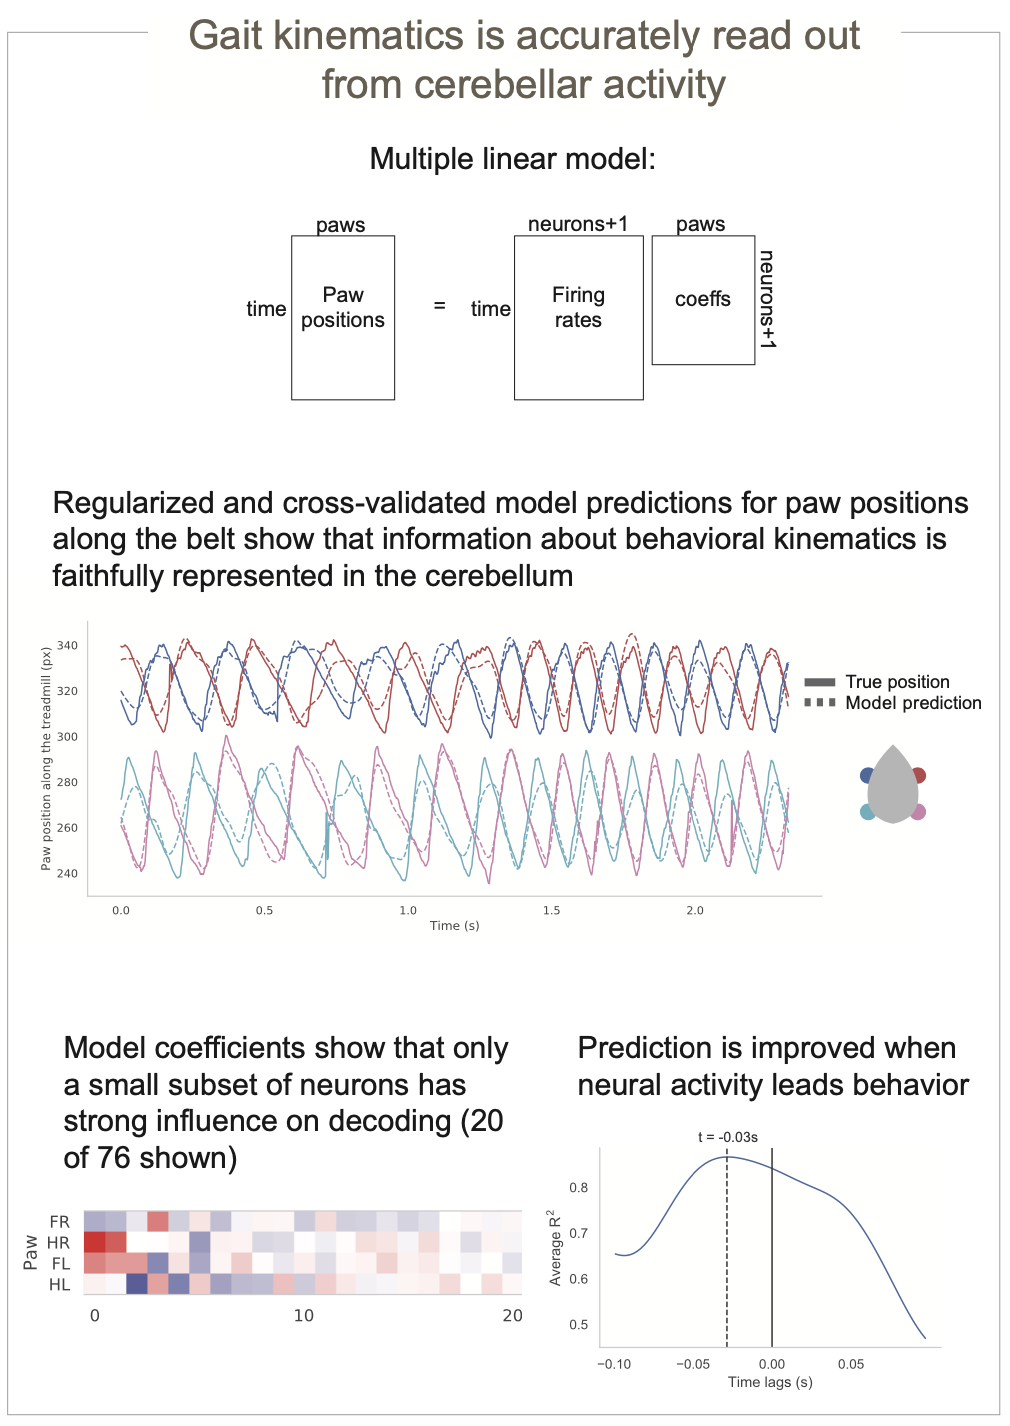
\includegraphics[width=.9\linewidth]{Chapters/Figures/chapter5/npx_decoder.png}
    \caption{Kinematics can be readout from cerebellar population instantaneous firing rates}
    \label{fig:enter-label}
\end{figure}


\subsection{Neural trajectories in neural populations have different complexity in mossy fibers and Purkinje cells}

\begin{figure}
    \centering
    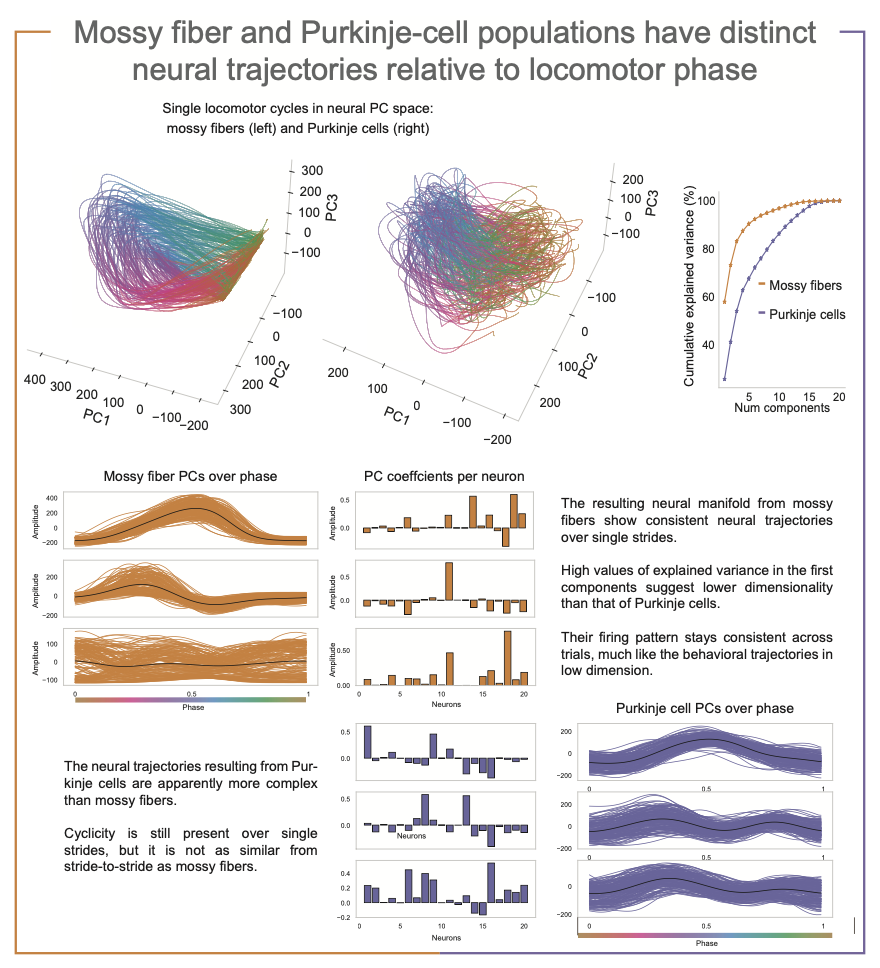
\includegraphics[width=0.99\linewidth]{Chapters/Figures/chapter5/neural_trajectories.png}
    \caption{Enter Caption}
    \label{fig:manifolds}
\end{figure}


\subsection{A conceptual hypothesis of cerebellar processing during locomotion}

\section{Discussion}

\section{Methods}
\subsection{Task and experimental design}
\subsection{Neuropixels}
\subsection{Recordings}
\subsection{Histology}
\subsection{Sorting individual units from raw data}
\subsection{Cell type identification}



